%\documentclass[paper=a4, fontsize=12pt]{scrartcl}
%\usepackage[T1]{fontenc}
%\usepackage{fourier}

%\usepackage[english]{babel}															% English language/hyphenation
%\usepackage[protrusion=true,expansion=true]{microtype}	
%\usepackage{amsmath,amsfonts,amsthm} % Math packages
%\usepackage[pdftex]{graphicx}	
%\usepackage{url}
%\usepackage{fancyhdr}

%%% Custom sectioning
%\usepackage{sectsty}
%\allsectionsfont{\centering \normalfont\scshape}


\documentclass[12pt]{article}

%\usepackage{a4wide}
\usepackage{times}
\usepackage{graphicx}
\usepackage{float}

%%% Custom headers/footers (fancyhdr package)
%\usepackage{fancyhdr}
%\pagestyle{fancyplain}
%\fancyhead{}											% No page header
%\fancyfoot[L]{}											% Empty 
%\fancyfoot[C]{}											% Empty
%\fancyfoot[R]{\thepage}									% Pagenumbering
%\renewcommand{\headrulewidth}{0pt}			% Remove header underlines
%\renewcommand{\footrulewidth}{0pt}				% Remove footer underlines
%\setlength{\headheight}{13.6pt}


%%% Equation and float numbering
%\numberwithin{equation}{section}		% Equationnumbering: section.eq#
%\numberwithin{figure}{section}			% Figurenumbering: section.fig#
%\numberwithin{table}{section}				% Tablenumbering: section.tab#


%%% Maketitle metadata
\newcommand{\horrule}[1]{\rule{\linewidth}{#1}} 	% Horizontal rule

\title{
	%\vspace{-1in} 	
	\usefont{OT1}{bch}{b}{n}
	\normalfont \normalsize \textsc{University of the Witwatersrand} \\ [35pt]	
\begin{figure}[h]
\centering

\includegraphics[width=0.5\linewidth]{photo}
\label{fig:photo}
\end{figure}	
	\horrule{0.5pt} \\[0.4cm]
	\huge Project Report \\
	Advanced Analysis of Algorithms\\
	\horrule{2pt} \\[0.5cm]
}
\author{Sibusiso Mthethwa (570088) \and Liam Pulles (855442) \and Tshepiso Molobi (748877)}

\date{31 October 2016}


%%% Begin document
\begin{document}
\maketitle
\tableofcontents
\newpage
\section{Introduction}
\subsection{Aim and Objective}
Determining the relative measurement of an algorithm from theory, and comparing them to reality is one decisive idea in computer science. With this we can decide if the algorithm solution if practical or not. Provided that it is indeed practical, we will thus try to identify the points within the problem field that can be successfully used before exhausting the system. Consequently, implementing a Backtracking algorithm using java. The Backtracking algorithm will be used to solve the partially solved diverse Sudoku puzzles reserved in the database. To implement and test the Backtracking algorithm in relation to solving Sudoku puzzles given various number of empty spaces and of course these puzzles are of different arrangements. We will justify the theoretical analysis of the algorithm. A number of experiments will be conducted on the algorithm to measure the performance of the algorithm, and comparisons with the theoretical analysis will be made. With the number of empty spaces, we will do the Emperical analysis of the backtracking algorithm.

\subsection{Problem Statement}
We want to determine the complexity of our backtracking algorithm. We have done a theoretical analysis of our algorithm, but we need to see if this holds true in reality. An Empirical analysis on our implementation of the backtracking algorithm will be done, to see if the actual complexity conforms to our theoretical complexity. 

\section{Theoretical Background}
\subsection{Sudoku Principles}
Sudoku is a ralational and insightful puzzle, and to it the obejective is to pack a 9 by 9 grid with numbers such that every column, every row, and every 3 by 3 subgrid has all digits from 1 to 9 appearing precisely once. Each grid has an initial state with some number of cells having digits assigned to them.
\subsection{The Backtracking Algorithm}
The backtracking algorithm is an algorithm with common qualities with that of the brute force algorithm which is uses a lot less memory. The brute force algorithm will find an empty cell, then find the smallest valid digit from 1 to 9, that is not equal to any digit in the present space, column or row. Provided the digit is valid, the current empty space will be assigned this digit. This algorithm will be recursively called. If no valid digit is found, the algorithm will be called recursively while backtracking if necessary.

\section{Theoretical Analysis}
A single cell belonging to a Sudoku puzzle contains a unique digit column wise and row wise. Provided a cell with a digit, each cell corresponding to that cell column wise or row wise is prohibited from having the exact number. This restriction we will be verified by a method in relation to how a given Sudoku puzzle is in memory represented. The backtracking algorithm is performed on this logic puzzle, such that if we reach a dead-end while solving the puzzle, then the algorithm will reverse the move and it will try to explore other different paths that have not been traveled until it gets the solution to the puzzle.\\\\
In general terms, the algorithm has a complexity that is highly dependent on how complete the given puzzle is, where we consider the number of empty spaces in the Sudoku puzzle. Below are the cases we will look into\\\\
Best Case:\\
The best case scenario is when the path chosen from the beggining to the end is correct, thus the algorithm does not need to backtrack.\\\\
Worst Case:\\
In the worst case scenario all the paths have to be traveled before getting to the final arrangement of the Sudoku elements, as a result the algorithm backtracks at every chosen digit.


\subsection{Time Complexity}
Worst Case:
Let j denote the number of empty cells in a given Sudoku puzzle. We will use undirected acyclic trees to structure our solution explanation. For each empty cell, there exists 9 possibilities. We will have 9 nodes added to the tree, with each new node representing a possible solution to a cell first looked into. These nodes will be connected to our arbitrary root node through an addition of 9 edges. Moving to the second empty cell which will as well have 9 possibilities. We add another level to our tree through adding 9 nodes to all the nodes in level 1. Continuing in this way, we will get to a problem that comes about by a brute force approach. Our backtracking algorithm will take action in way similar to that of the depth first search algorithm upon the constructed tree. The algorithm will go over one branch of the tree up to violating a condition under the Sudoku Fundamentals where it will backtrack and try a different tree branch. Coondidering a tree of n nodes and m edges, the Depth First Search has a complexity of O(n+m). Now looking into our problem, \[n = 9^{j}\] given 9 nodes at every level for each of the nodes. Assuming that all the provided Sudoku puzzles may not have the number clues below 17, then the max number of empty spaces (j) is 81 - 17 = 64. We in the worst case take our upper bound to be \[O(9^{64})\] since j can never go beyond 64.\\\\        
Best Case:\\
The best case for this algorithm is that it discovers the solution to the problem the very first time through, that it won't have tp backtrack at all. This means that every predicted digit by the algorithm, this being the first guess is well found and thus correct with the algorithm not having to backtrack. This does not by any chance depend on the number of empty spaces. Since the algorithm never backtracks, the first node of the tree is the only node to be iterated through. This results in the complexity \[n=1^{j}\], j = 64 is the upper bound. \[1^{64} = 1\], thus we can conclude that O(1) is the complexity in the best case.


\section{Experiment}

\subsection{Experimental Methodology}
Begin a Java program that has the functionalities below:\\
\begin{itemize}
	\item Allow input and storing of a Sudoku puzzle with various number of empty spaces. These puzzles will read at random from a database.
	\item Use the Backtracking Algorithm to find a solution to a given Sudoku puzzle.
	\item Measure the average time it took the Backtracking Algorithm to find a solution Sudoku puzzle. 
\end{itemize}
For accuracy's sake the experiment was done multiple times. And the graphs of time vs number of empty spaces was obtained to make the performance of the backtracking algorithm feasible enough, that we can be able to conclude on its complexity.
\subsection{Apparatus}
\begin{itemize}
	\item NetBeans IDE - Java Code
	\item RAM (4 GB)
	\item Linux Operating System (Arch, latest linux kernel) 
	\item Processor (Core i5 3.8GHz) 
\end{itemize}

\section{Results}	

\subsection{Presentation of Results}
The results presented below are that of the experiments that were conducted and their graphs.

\begin{figure}[H]
\centering
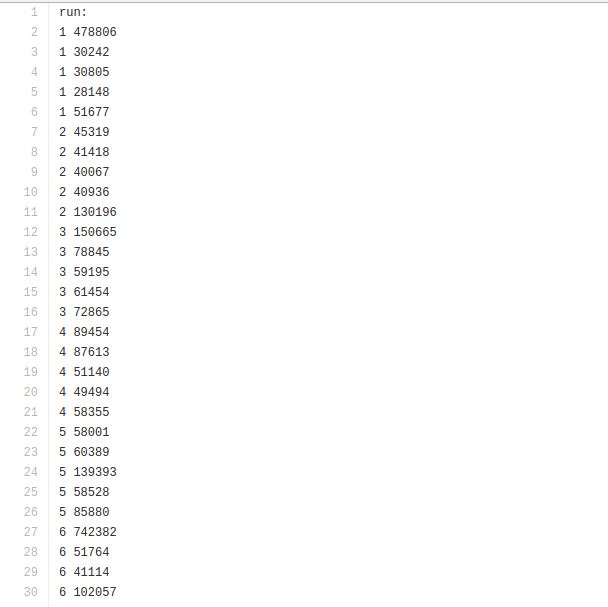
\includegraphics[width=0.7\linewidth]{1-30.jpg}
\label{fig:1-30}
\end{figure}

\begin{figure}[H]
\centering
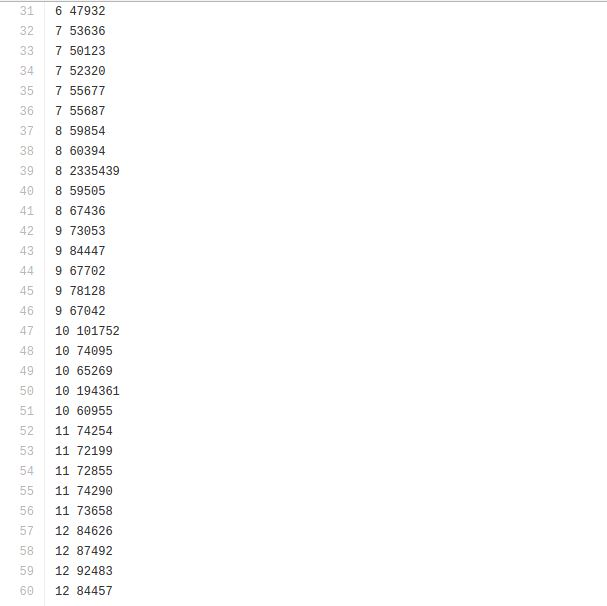
\includegraphics[width=0.7\linewidth]{31-61.jpg}
\label{fig:31-61}
\end{figure}

\begin{figure}[H]
\centering
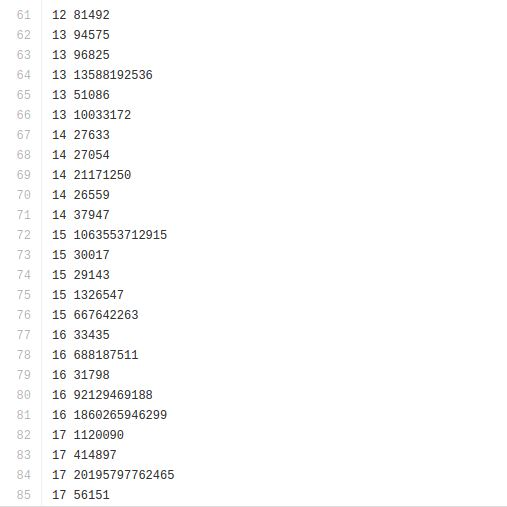
\includegraphics[width=0.7\linewidth]{61-85.jpg}
\label{fig:61-85}
\end{figure}

\begin{figure}[H]
\centering
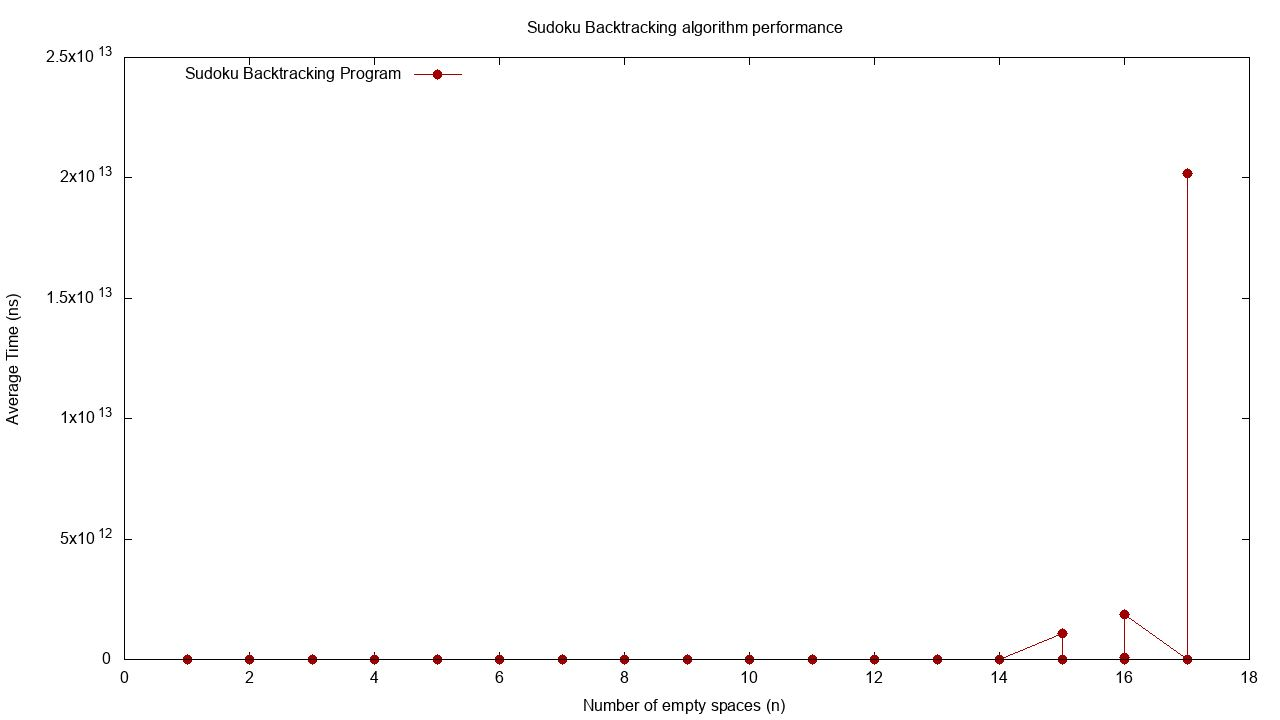
\includegraphics[width=0.7\linewidth]{graph.jpg}
\label{fig:graph}
\end{figure}

\subsection{Results Analysis}
The results that appear in fig:1-30, fig:31-61 and fig:61-85 were gathered from the experiments that were performed. The results show two columns with the first one being the number of empty blocks on the Sudoku board.The second one represents the time taken(in nano seconds) to solve the board.

From the results that were gathered a graph was drawn up to show the complexity of the algorithm as the number of empty blocks increases.
The graph depicts what seems to be an exponential growth, which as hypothesized suggests that as the input size of the empty blocks increases, more time is needed to solve the Sudoku puzzles. 

\subsection{Results in Relation to Theory}
This section is dedicated to comparing the complexity of the experiments by the backtracking algorithm to the theoretical complexity of the algorithm that we conducted. The graph shows that the average time of the backtracking in comparison to the the number of the empty spaces.
If we were to take into consideration direct cell comparisons as a basic operation, it can be shown that the time complexity is bounded
above by O($9^j$) in the worst case.
In the best case we have complexity of O(1). This correlates to the empirical complexity that we hypothesized, although the results would have been more accurate given more empty spaces which would require more time. Due to the time constraints the results were compiled until 17 empty spaces.   

\section{Conclusion}
In conclusion we can see that the analysis of Sudoku contains many complexities, and that given the enormity of the state space, the number of tests that could be performed in our alloted time was limited.

However, it is clear to see that the performance in the best and worst case of sudoku vary astronomically.

The algorithm could be improved further by sorting possible moves so as moves where only one number for a position is possible are done first. These would be guarenteed moves. And even if only two moves are possible for a position, the amount of backtracking would still be reduced - and the benefits down the line of recursive calls would be enormous. It could increase the complexity of our best and worst case slightly due to the sorting algorithm, but it would reduce the average case substantially. We implemented this program and for the interested reader the neccesary functions can be found in the Optimized.java class, which is not currently used.

Other improvements might include a dynamic programming element, which might be a structure in memory which holds moves already found. The list of moves would have to be removed and added to with recursive calls and bactraking respectively, but is not out of the realm of possibility and may reduce complexity and increase performance in the long run.

\section{Group Work Allotment}
The work allotment is (generally) as follows:

Liam Pulles
\begin{itemize}
\item Code (80\%)
\item Test Design and Result generation
\item Graph section
\item Conclusion section
\end{itemize}

Sibusiso Mthethwa
\begin{itemize}
\item Code (10\%)
\item Results section
\end{itemize}

Tshepiso Molobi
\begin{itemize}
\item Code (10\%)
\item Introduction section
\item Background theory section
\item Theoretical analysis section
\item Experiment section
\end{itemize}  
\end{document}
